\documentclass{standalone}
\usepackage{tikz}
\usetikzlibrary{patterns, positioning}


\begin{document}
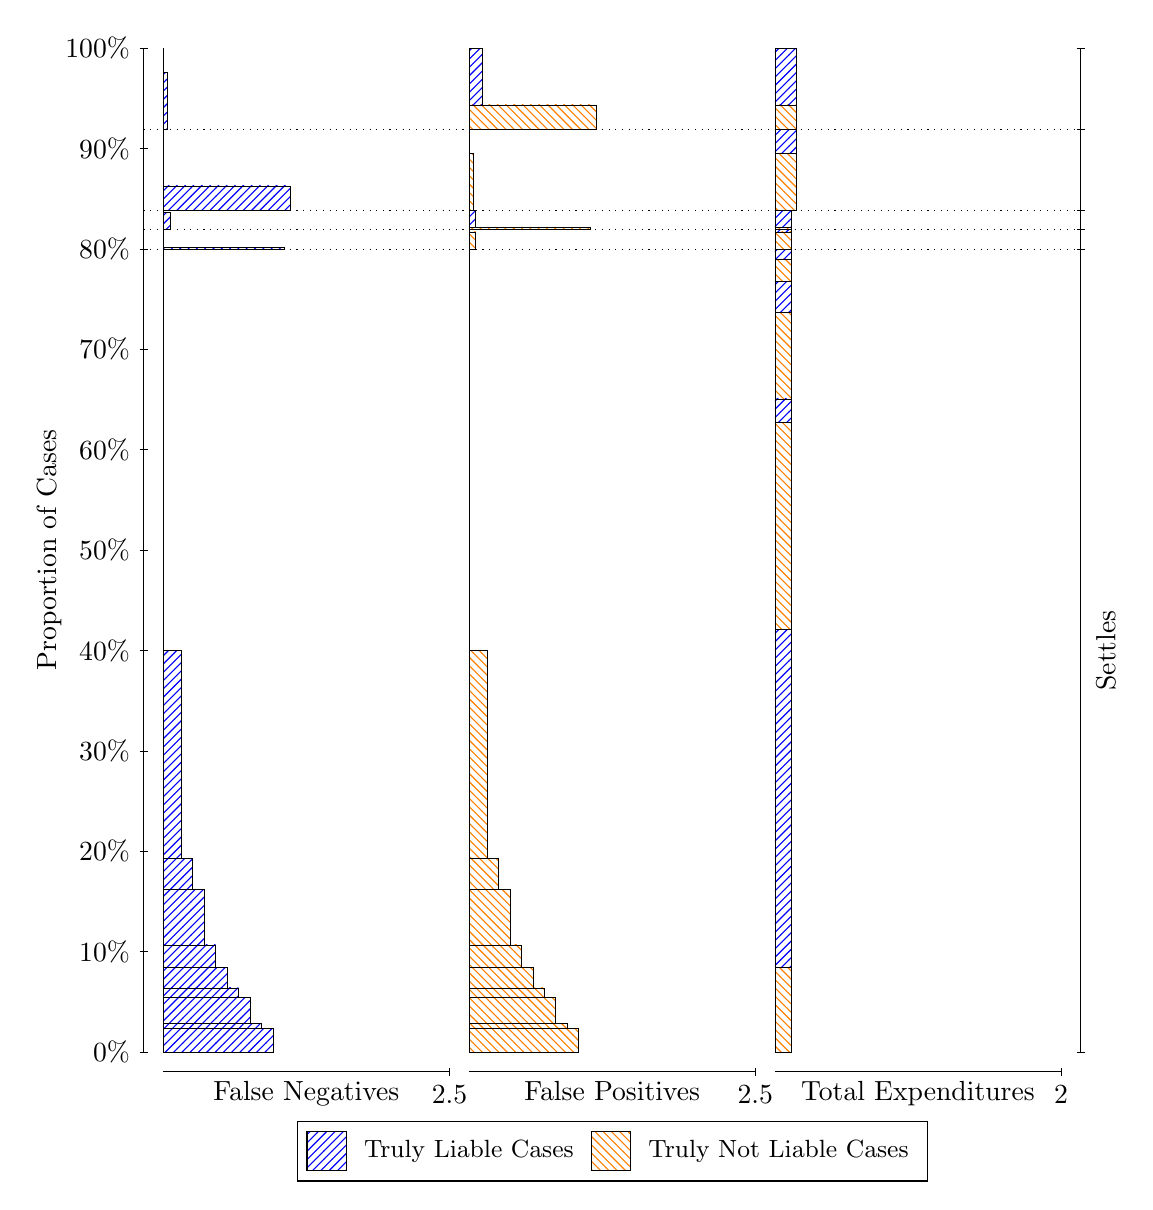
\begin{tikzpicture}
\draw[black, very thin] (1.5,1.75) -- (1.5,14.5);
\node[rotate=90, text=black, anchor=center] at (0.3, 8.125) {Proportion of Cases};
\draw[black, very thin] (1.45,1.75) -- (1.55,1.75);
\node[text=black, anchor=east] at (1.45, 1.75) {0\%};
\draw[black, very thin] (1.45,3.025) -- (1.55,3.025);
\node[text=black, anchor=east] at (1.45, 3.025) {10\%};
\draw[black, very thin] (1.45,4.3) -- (1.55,4.3);
\node[text=black, anchor=east] at (1.45, 4.3) {20\%};
\draw[black, very thin] (1.45,5.575) -- (1.55,5.575);
\node[text=black, anchor=east] at (1.45, 5.575) {30\%};
\draw[black, very thin] (1.45,6.85) -- (1.55,6.85);
\node[text=black, anchor=east] at (1.45, 6.85) {40\%};
\draw[black, very thin] (1.45,8.125) -- (1.55,8.125);
\node[text=black, anchor=east] at (1.45, 8.125) {50\%};
\draw[black, very thin] (1.45,9.4) -- (1.55,9.4);
\node[text=black, anchor=east] at (1.45, 9.4) {60\%};
\draw[black, very thin] (1.45,10.675) -- (1.55,10.675);
\node[text=black, anchor=east] at (1.45, 10.675) {70\%};
\draw[black, very thin] (1.45,11.95) -- (1.55,11.95);
\node[text=black, anchor=east] at (1.45, 11.95) {80\%};
\draw[black, very thin] (1.45,13.225) -- (1.55,13.225);
\node[text=black, anchor=east] at (1.45, 13.225) {90\%};
\draw[black, very thin] (1.45,14.5) -- (1.55,14.5);
\node[text=black, anchor=east] at (1.45, 14.5) {100\%};

\draw[black, very thin] (13.4,1.75) -- (13.4,14.5);
\draw[black, very thin] (13.35,1.75) -- (13.45,1.75);
\node[anchor=west] at (13.35, 1.75) {};
\draw[black, very thin] (13.35,11.945) -- (13.45,11.945);
\node[anchor=west] at (13.35, 11.945) {};
\draw[black, very thin] (13.35,12.194) -- (13.45,12.194);
\node[anchor=west] at (13.35, 12.194) {};
\draw[black, very thin] (13.35,12.442) -- (13.45,12.442);
\node[anchor=west] at (13.35, 12.442) {};
\draw[black, very thin] (13.35,13.471) -- (13.45,13.471);
\node[anchor=west] at (13.35, 13.471) {};
\draw[black, very thin] (13.35,14.5) -- (13.45,14.5);
\node[anchor=west] at (13.35, 14.5) {};

\draw[black, very thin, pattern color=blue, pattern=north east lines] (1.75,1.75) rectangle (3.1398,2.0469);
\draw[black, very thin, pattern color=blue, pattern=north east lines] (1.75,2.0469) rectangle (2.9944,2.1177);
\draw[black, very thin, pattern color=blue, pattern=north east lines] (1.75,2.1177) rectangle (2.8491,2.4406);
\draw[black, very thin, pattern color=blue, pattern=north east lines] (1.75,2.4406) rectangle (2.7037,2.5633);
\draw[black, very thin, pattern color=blue, pattern=north east lines] (1.75,2.5633) rectangle (2.5584,2.8279);
\draw[black, very thin, pattern color=blue, pattern=north east lines] (1.75,2.8279) rectangle (2.4131,3.1113);
\draw[black, very thin, pattern color=blue, pattern=north east lines] (1.75,3.1113) rectangle (2.2678,3.8167);
\draw[black, very thin, pattern color=blue, pattern=north east lines] (1.75,3.8167) rectangle (2.1224,4.2124);
\draw[black, very thin, pattern color=blue, pattern=north east lines] (1.75,4.2124) rectangle (1.9771,6.8474);
\draw[black, very thin, pattern color=orange, pattern=north west lines] (1.75,6.8474) rectangle (1.75,11.945);
\draw[black, very thin, pattern color=blue, pattern=north east lines] (1.75,11.945) rectangle (3.2851,11.972);
\draw[black, very thin, pattern color=orange, pattern=north west lines] (1.75,11.972) rectangle (1.75,12.194);
\draw[black, very thin, pattern color=blue, pattern=north east lines] (1.75,12.194) rectangle (1.8318,12.415);
\draw[black, very thin, pattern color=orange, pattern=north west lines] (1.75,12.415) rectangle (1.75,12.442);
\draw[black, very thin, pattern color=blue, pattern=north east lines] (1.75,12.442) rectangle (3.3668,12.749);
\draw[black, very thin, pattern color=orange, pattern=north west lines] (1.75,12.749) rectangle (1.75,13.471);
\draw[black, very thin, pattern color=blue, pattern=north east lines] (1.75,13.471) rectangle (1.8045,14.194);
\draw[black, very thin, pattern color=orange, pattern=north west lines] (1.75,14.194) rectangle (1.75,14.5);
\draw[black, very thin, pattern color=orange, pattern=north west lines] (5.6333,1.75) rectangle (7.0231,2.0468);
\draw[black, very thin, pattern color=orange, pattern=north west lines] (5.6333,2.0468) rectangle (6.8777,2.1177);
\draw[black, very thin, pattern color=orange, pattern=north west lines] (5.6333,2.1177) rectangle (6.7324,2.4405);
\draw[black, very thin, pattern color=orange, pattern=north west lines] (5.6333,2.4405) rectangle (6.5871,2.5633);
\draw[black, very thin, pattern color=orange, pattern=north west lines] (5.6333,2.5633) rectangle (6.4417,2.8279);
\draw[black, very thin, pattern color=orange, pattern=north west lines] (5.6333,2.8279) rectangle (6.2964,3.1113);
\draw[black, very thin, pattern color=orange, pattern=north west lines] (5.6333,3.1113) rectangle (6.1511,3.8167);
\draw[black, very thin, pattern color=orange, pattern=north west lines] (5.6333,3.8167) rectangle (6.0057,4.2125);
\draw[black, very thin, pattern color=orange, pattern=north west lines] (5.6333,4.2125) rectangle (5.8604,6.8475);
\draw[black, very thin, pattern color=blue, pattern=north east lines] (5.6333,6.8475) rectangle (5.6333,11.945);
\draw[black, very thin, pattern color=orange, pattern=north west lines] (5.6333,11.945) rectangle (5.7151,12.166);
\draw[black, very thin, pattern color=blue, pattern=north east lines] (5.6333,12.166) rectangle (5.6333,12.194);
\draw[black, very thin, pattern color=orange, pattern=north west lines] (5.6333,12.194) rectangle (7.1684,12.221);
\draw[black, very thin, pattern color=blue, pattern=north east lines] (5.6333,12.221) rectangle (5.7151,12.442);
\draw[black, very thin, pattern color=orange, pattern=north west lines] (5.6333,12.442) rectangle (5.6878,13.165);
\draw[black, very thin, pattern color=blue, pattern=north east lines] (5.6333,13.165) rectangle (5.6333,13.471);
\draw[black, very thin, pattern color=orange, pattern=north west lines] (5.6333,13.471) rectangle (7.2502,13.778);
\draw[black, very thin, pattern color=blue, pattern=north east lines] (5.6333,13.778) rectangle (5.7968,14.5);
\draw[black, very thin, pattern color=orange, pattern=north west lines] (9.5167,1.75) rectangle (9.721,2.8279);
\draw[black, very thin, pattern color=blue, pattern=north east lines] (9.5167,2.8279) rectangle (9.721,7.112);
\draw[black, very thin, pattern color=orange, pattern=north west lines] (9.5167,7.112) rectangle (9.721,9.7471);
\draw[black, very thin, pattern color=blue, pattern=north east lines] (9.5167,9.7471) rectangle (9.721,10.044);
\draw[black, very thin, pattern color=orange, pattern=north west lines] (9.5167,10.044) rectangle (9.721,11.145);
\draw[black, very thin, pattern color=blue, pattern=north east lines] (9.5167,11.145) rectangle (9.721,11.539);
\draw[black, very thin, pattern color=orange, pattern=north west lines] (9.5167,11.539) rectangle (9.721,11.822);
\draw[black, very thin, pattern color=blue, pattern=north east lines] (9.5167,11.822) rectangle (9.721,11.945);
\draw[black, very thin, pattern color=orange, pattern=north west lines] (9.5167,11.945) rectangle (9.721,12.166);
\draw[black, very thin, pattern color=blue, pattern=north east lines] (9.5167,12.166) rectangle (9.721,12.194);
\draw[black, very thin, pattern color=orange, pattern=north west lines] (9.5167,12.194) rectangle (9.721,12.221);
\draw[black, very thin, pattern color=blue, pattern=north east lines] (9.5167,12.221) rectangle (9.721,12.442);
\draw[black, very thin, pattern color=orange, pattern=north west lines] (9.5167,12.442) rectangle (9.7892,13.165);
\draw[black, very thin, pattern color=blue, pattern=north east lines] (9.5167,13.165) rectangle (9.7892,13.471);
\draw[black, very thin, pattern color=orange, pattern=north west lines] (9.5167,13.471) rectangle (9.7892,13.778);
\draw[black, very thin, pattern color=blue, pattern=north east lines] (9.5167,13.778) rectangle (9.7892,14.5);
\draw[black, dotted] (1.5,11.945) -- (13.4,11.945);
\draw[black, dotted] (1.5,12.194) -- (13.4,12.194);
\draw[black, dotted] (1.5,12.442) -- (13.4,12.442);
\draw[black, dotted] (1.5,13.471) -- (13.4,13.471);
\draw[black, very thin] (1.75,1.5) -- (5.3833,1.5);
\node[text=black, anchor=north] at (3.5667, 1.5) {False Negatives};
\draw[black, very thin] (5.3833,1.45) -- (5.3833,1.55);
\node[text=black, anchor=north] at (5.3833, 1.45) {2.5};

\draw[black, very thin] (5.6333,1.5) -- (9.2667,1.5);
\node[text=black, anchor=north] at (7.45, 1.5) {False Positives};
\draw[black, very thin] (9.2667,1.45) -- (9.2667,1.55);
\node[text=black, anchor=north] at (9.2667, 1.45) {2.5};

\draw[black, very thin] (9.5167,1.5) -- (13.15,1.5);
\node[text=black, anchor=north] at (11.333, 1.5) {Total Expenditures};
\draw[black, very thin] (13.15,1.45) -- (13.15,1.55);
\node[text=black, anchor=north] at (13.15, 1.45) {2};

\node[text=black, centered, rotate=90] at (13.72, 6.8475) {Settles};





\draw (7.449999999999999,1.5) node[draw=none] (baseCoordinate) {};
\begin{scope}[align=center]
        \matrix[scale=0.5, draw=black, below=0.5cm of baseCoordinate, nodes={draw}, column sep=0.1cm]{
            \node[rectangle, draw, minimum width=0.5cm, minimum height=0.5cm, pattern color=blue, pattern=north east lines] {}; &
            \node[draw=none, font=\small, text=black] (B) {Truly Liable Cases}; &
            \node[rectangle, draw, minimum width=0.5cm, minimum height=0.5cm, pattern color=orange, pattern=north west lines] {}; &
            \node[draw=none, font=\small, text=black] (B) {Truly Not Liable Cases}; \\
            };
\end{scope}

\end{tikzpicture}
\end{document}